% The Computer Simulation of Molecular Dynamics
% Nan Dun <dun@logos.ic.i.u-tokyo.ac.jp>


%% bare_jrnl_compsoc.tex
%% V1.3
%% 2007/01/11
%% by Michael Shell
%% See:
%% http://www.michaelshell.org/
%% for current contact information.
%%
%% This is a skeleton file demonstrating the use of IEEEtran.cls
%% (requires IEEEtran.cls version 1.7 or later) with an IEEE Computer
%% Society journal paper.
%%
%% Support sites:
%% http://www.michaelshell.org/tex/ieeetran/
%% http://www.ctan.org/tex-archive/macros/latex/contrib/IEEEtran/
%% and
%% http://www.ieee.org/

\documentclass[a4paper,10pt,technote,compsoc,onecolumn]{IEEEtran}

% Centering figure captions
\makeatletter
\long\def\@makecaption#1#2{\ifx\@captype\@IEEEtablestring%
\footnotesize\begin{center}{\normalfont\footnotesize #1}\\
{\normalfont\footnotesize\scshape #2}\end{center}%
\@IEEEtablecaptionsepspace
\else
\@IEEEfigurecaptionsepspace
\setbox\@tempboxa\hbox{\normalfont\footnotesize {#1.}~~ #2}%
\ifdim \wd\@tempboxa >\hsize%
\setbox\@tempboxa\hbox{\normalfont\footnotesize {#1.}~~ }%
\parbox[t]{\hsize}{\normalfont\footnotesize \noindent\unhbox\@tempboxa#2}%
\else
\hbox to\hsize{\normalfont\footnotesize\hfil\box\@tempboxa\hfil}\fi\fi}
\makeatother

% *** GRAPHICS RELATED PACKAGES ***
%
\ifCLASSINFOpdf
  % \usepackage[pdftex]{graphicx}
  % declare the path(s) where your graphic files are
  % \graphicspath{{../pdf/}{../jpeg/}}
  % and their extensions so you won't have to specify these with
  % every instance of \includegraphics
  % \DeclareGraphicsExtensions{.pdf,.jpeg,.png}
\else
  % or other class option (dvipsone, dvipdf, if not using dvips). graphicx
  % will default to the driver specified in the system graphics.cfg if no
  % driver is specified.
  % \usepackage[dvips]{graphicx}
  % declare the path(s) where your graphic files are
  % \graphicspath{{../eps/}}
  % and their extensions so you won't have to specify these with
  % every instance of \includegraphics
  % \DeclareGraphicsExtensions{.eps}
\fi
% graphicx was written by David Carlisle and Sebastian Rahtz. It is
% required if you want graphics, photos, etc. graphicx.sty is already
% installed on most LaTeX systems. The latest version and documentation can
% be obtained at: 
% http://www.ctan.org/tex-archive/macros/latex/required/graphics/
% Another good source of documentation is "Using Imported Graphics in
% LaTeX2e" by Keith Reckdahl which can be found as epslatex.ps or
% epslatex.pdf at: http://www.ctan.org/tex-archive/info/
%
% latex, and pdflatex in dvi mode, support graphics in encapsulated
% postscript (.eps) format. pdflatex in pdf mode supports graphics
% in .pdf, .jpeg, .png and .mps (metapost) formats. Users should ensure
% that all non-photo figures use a vector format (.eps, .pdf, .mps) and
% not a bitmapped formats (.jpeg, .png). IEEE frowns on bitmapped formats
% which can result in "jaggedy"/blurry rendering of lines and letters as
% well as large increases in file sizes.
%
% You can find documentation about the pdfTeX application at:
% http://www.tug.org/applications/pdftex

\usepackage[cmex10]{amsmath}
\usepackage{amssymb}
\interdisplaylinepenalty=2500
\usepackage{algorithmic}
\usepackage{array}


%\usepackage{eqparbox}
% Also of notable interest is Scott Pakin's eqparbox package for creating
% (automatically sized) equal width boxes - aka "natural width parboxes".
% Available at:
% http://www.ctan.org/tex-archive/macros/latex/contrib/eqparbox/

% *** SUBFIGURE PACKAGES ***
%\ifCLASSOPTIONcompsoc
%\usepackage[tight,normalsize,sf,SF]{subfigure}
%\else
%\usepackage[tight,footnotesize]{subfigure}
%\fi
% subfigure.sty was written by Steven Douglas Cochran. This package makes it
% easy to put subfigures in your figures. e.g., "Figure 1a and 1b". For IEEE
% work, it is a good idea to load it with the tight package option to reduce
% the amount of white space around the subfigures. Computer Society papers
% use a larger font and \sffamily font for their captions, hence the
% additional options needed under compsoc mode. subfigure.sty is already
% installed on most LaTeX systems. The latest version and documentation can
% be obtained at:
% http://www.ctan.org/tex-archive/obsolete/macros/latex/contrib/subfigure/
% subfigure.sty has been superceeded by subfig.sty.


%\ifCLASSOPTIONcompsoc
%  \usepackage[caption=false]{caption}
%  \usepackage[font=normalsize,labelfont=sf,textfont=sf]{subfig}
%\else
%  \usepackage[caption=false]{caption}
%  \usepackage[font=footnotesize]{subfig}
%\fi
% subfig.sty, also written by Steven Douglas Cochran, is the modern
% replacement for subfigure.sty. However, subfig.sty requires and
% automatically loads Axel Sommerfeldt's caption.sty which will override
% IEEEtran.cls handling of captions and this will result in nonIEEE style
% figure/table captions. To prevent this problem, be sure and preload
% caption.sty with its "caption=false" package option. This is will preserve
% IEEEtran.cls handing of captions. Version 1.3 (2005/06/28) and later 
% (recommended due to many improvements over 1.2) of subfig.sty supports
% the caption=false option directly:
%\ifCLASSOPTIONcompsoc
%  \usepackage[caption=false,font=normalsize,labelfont=sf,textfont=sf]{subfig}
%\else
%  \usepackage[caption=false,font=footnotesize]{subfig}
%\fi
%
% The latest version and documentation can be obtained at:
% http://www.ctan.org/tex-archive/macros/latex/contrib/subfig/
% The latest version and documentation of caption.sty can be obtained at:
% http://www.ctan.org/tex-archive/macros/latex/contrib/caption/


%\usepackage{stfloats}
% stfloats.sty was written by Sigitas Tolusis. This package gives LaTeX2e
% the ability to do double column floats at the bottom of the page as well
% as the top. (e.g., "\begin{figure*}[!b]" is not normally possible in
% LaTeX2e). It also provides a command:
%\fnbelowfloat
% to enable the placement of footnotes below bottom floats (the standard
% LaTeX2e kernel puts them above bottom floats). This is an invasive package
% which rewrites many portions of the LaTeX2e float routines. It may not work
% with other packages that modify the LaTeX2e float routines. The latest
% version and documentation can be obtained at:
% http://www.ctan.org/tex-archive/macros/latex/contrib/sttools/
% Documentation is contained in the stfloats.sty comments as well as in the
% presfull.pdf file. Do not use the stfloats baselinefloat ability as IEEE
% does not allow \baselineskip to stretch. Authors submitting work to the
% IEEE should note that IEEE rarely uses double column equations and
% that authors should try to avoid such use. Do not be tempted to use the
% cuted.sty or midfloat.sty packages (also by Sigitas Tolusis) as IEEE does
% not format its papers in such ways.




%\ifCLASSOPTIONcaptionsoff
%  \usepackage[nomarkers]{endfloat}
% \let\MYoriglatexcaption\caption
% \renewcommand{\caption}[2][\relax]{\MYoriglatexcaption[#2]{#2}}
%\fi
% endfloat.sty was written by James Darrell McCauley and Jeff Goldberg.
% This package may be useful when used in conjunction with IEEEtran.cls'
% captionsoff option. Some IEEE journals/societies require that submissions
% have lists of figures/tables at the end of the paper and that
% figures/tables without any captions are placed on a page by themselves at
% the end of the document. If needed, the draftcls IEEEtran class option or
% \CLASSINPUTbaselinestretch interface can be used to increase the line
% spacing as well. Be sure and use the nomarkers option of endfloat to
% prevent endfloat from "marking" where the figures would have been placed
% in the text. The two hack lines of code above are a slight modification of
% that suggested by in the endfloat docs (section 8.3.1) to ensure that
% the full captions always appear in the list of figures/tables - even if
% the user used the short optional argument of \caption[]{}.
% IEEE papers do not typically make use of \caption[]'s optional argument,
% so this should not be an issue. A similar trick can be used to disable
% captions of packages such as subfig.sty that lack options to turn off
% the subcaptions:
% For subfig.sty:
% \let\MYorigsubfloat\subfloat
% \renewcommand{\subfloat}[2][\relax]{\MYorigsubfloat[]{#2}}
% For subfigure.sty:
% \let\MYorigsubfigure\subfigure
% \renewcommand{\subfigure}[2][\relax]{\MYorigsubfigure[]{#2}}
% However, the above trick will not work if both optional arguments of
% the \subfloat/subfig command are used. Furthermore, there needs to be a
% description of each subfigure *somewhere* and endfloat does not add
% subfigure captions to its list of figures. Thus, the best approach is to
% avoid the use of subfigure captions (many IEEE journals avoid them anyway)
% and instead reference/explain all the subfigures within the main caption.
% The latest version of endfloat.sty and its documentation can obtained at:
% http://www.ctan.org/tex-archive/macros/latex/contrib/endfloat/
%
% The IEEEtran \ifCLASSOPTIONcaptionsoff conditional can also be used
% later in the document, say, to conditionally put the References on a 
% page by themselves.

\usepackage{hyperref}
\usepackage{acronym}
\usepackage{booktabs}
\usepackage{colortbl}
\usepackage{units}
\usepackage{tikz}
\usetikzlibrary{shapes,arrows}
\usepackage{pgfplots}
\usepackage{listings}
\usepackage{courier}
\usepackage{array}

\hypersetup{
  bookmarks=true,
  pdfborder={0 0 0},
  colorlinks=true,
  linkcolor=magenta,
  citecolor=black,%green
  filecolor=magenta,
  urlcolor=cyan,
}

% correct bad hyphenation here
\hyphenation{op-tical net-works semi-conduc-tor}
%\hyphenpenalty=10000

\graphicspath{{figures/}}
\def\figwidth{0.75\textwidth}
\def\figheight{0.4\textwidth}

\pgfplotsset{width=\figwidth, height=\figheight, compat=1.3,
 x label style={font=\small}, y label style={font=\small},
 x tick label style={font=\footnotesize},
 y tick label style={font=\footnotesize},
 legend style={font=\small}}

\lstset{%
  language=C,
  basicstyle=\small\ttfamily,
  frame=lines,
  morekeywords={var, real, domain, forall, coforall, begin, cobegin, in, on, %
    record, sync, bool}
}

\newcommand{\ic}[1]{\tt\small #1}
\newcommand{\ie}{i.\,e., }
\newcommand{\Ie}{I.\,e., }
\newcommand{\eg}{e.\,g., }
\newcommand{\Eg}{E.\,g., }

\numberwithin{equation}{section}

\newcommand{\tabrowcolor}{\rowcolor[gray]{.9}}

\begin{document}
\title{Molecular Dynamics Simulation in Chapel}

\author{{\rm Nan Dun} \\ 
{\it Department of Information and Communication} \\
{\it The University of Tokyo, Tokyo, Japan} \\
{\it Email: \href{mailto:dun@logos.ic.i.u-tokyo.ac.jp}{dun@logos.ic.i.u-tokyo.ac.jp}}
        % <-this % stops a space
%\IEEEcompsocitemizethanks{
%\IEEEcompsocthanksitem Department
%of Information and Communication, the University of Tokyo, Tokyo,
%Japan, 1138656.\protect\\
% note need leading \protect in front of \\ to get a newline within \thanks as
% \\ is fragile and will error, could use \hfil\break instead.
%E-mail: \href{mailto:dun@logos.ic.i.u-tokyo.ac.jp}{dun@logos.ic.i.u-tokyo.ac.jp}
%}% <-this % stops a space
%\thanks{Manuscript revised}
}

\markboth{TECHNICAL NOTES, JST CREST, 2011}%
{Dun \MakeLowercase{\textit{et al.}}: Molecular Dynamics Simulation in Chapel}

%\IEEEcompsoctitleabstractindextext{%
%\begin{abstract}
%\boldmath
%The abstract goes here.
%\end{abstract}
% IEEEtran.cls defaults to using nonbold math in the Abstract.
% This preserves the distinction between vectors and scalars. However,
% if the journal you are submitting to favors bold math in the abstract,
% then you can use LaTeX's standard command \boldmath at the very start
% of the abstract to achieve this. Many IEEE journals frown on math
% in the abstract anyway. In particular, the Computer Society does
% not want either math or citations to appear in the abstract.

% Note that keywords are not normally used for peerreview papers.
%\begin{IEEEkeywords}
%Molecular dynamics, computer simulation, algorithms
%\end{IEEEkeywords}}


% make the title area
\maketitle

% To allow for easy dual compilation without having to reenter the
% abstract/keywords data, the \IEEEcompsoctitleabstractindextext text will
% not be used in maketitle, but will appear (i.e., to be "transported")
% here as \IEEEdisplaynotcompsoctitleabstractindextext when compsoc mode
% is not selected <OR> if conference mode is selected - because compsoc
% conference papers position the abstract like regular (non-compsoc)
% papers do!
\IEEEdisplaynotcompsoctitleabstractindextext
% \IEEEdisplaynotcompsoctitleabstractindextext has no effect when using
% compsoc under a non-conference mode.


% For peer review papers, you can put extra information on the cover
% page as needed:
% \ifCLASSOPTIONpeerreview
% \begin{center} \bfseries EDICS Category: 3-BBND \end{center}
% \fi
%
% For peerreview papers, this IEEEtran command inserts a page break and
% creates the second title. It will be ignored for other modes.
\IEEEpeerreviewmaketitle

% A
\acrodef{ASIC}[ASIC]{Application-Specific Integrated Circuit}

% C
\acrodef{CUDA}[CUDA]{Compute Unified Device Architecture}

% D
\acrodef{DARPA}[DARPA]{Defense Advanced Research Projects Agency}
\acrodef{DNA}[DNA]{Deoxyribonucleic Acid}

% F
\acrodef{FFT}[FFT]{Fast Fourier Transform}
\acrodef{FMM}[FMM]{Fast Multipole Method}

% G
\acrodef{GPU}[GPU]{Graphics Processing Unit}
\acrodef{GPGPU}[GPGPU]{General-Purpose Computing on Graphics Processing Unit}

% H
\acrodef{HPC}[HPC]{High Performance Computing}
\acrodef{HPCS}[HPCS]{High Productivity Computing Systems}

% K
\acrodef{KIFMM}[KIFMM]{Kernel-Independent FMM}

% L
\acrodef{LOC}[LOC]{Lines of Code}

% M
\acrodef{MD}[MD]{Molecular Dynamics}

% P
\acrodef{PGAS}[PGAS]{Partitioned Global Address Space}

% R
\acrodef{RNA}[RNA]{Ribonucleic Acid}

% S
\acrodef{SIMD}[SIMD]{Single Instruction Multiple Data}

% T
\acrodef{TBB}[TBB]{Threading Building Blocks}

% U
\acrodef{UPC}[UPC]{Unified Parallel C}


\section{Introduction}
\ac{MD} simulations compute the motions of individual molecules in motion of
solids, liquids, and gases. The key idea is {\em motion}, which describes how
positions, velocities, and orientations change with time~\cite{haile97mds,
furio97primer}. In \ac{MD}, the time evolution of a set of interacting atoms
is followed by integrating their equations of motion.

The laws of classical mechanics, \ie Newton's law, are applied in \ac{MD}.
\begin{equation}
  \vec{F}_i = m_i\vec{a}_i = m_i\frac{d\vec{v}_i}{dt} =
  m_i\frac{d^2\vec{r}_i}{dt^2}
\end{equation}
for each atom $i$ in a system constituted by $n$ atoms. Here, $m_i$ is the
atom mass, $\vec{a}_i$ is its acceleration, and $\vec{F}_i$ is the force
acting upon it.
Therefore, \ac{MD} is a {\em deterministic} approach. Given initial positions
and velocities, the evolution of the system in time is, in principle,
completely determined.  However, in practice, accumulation of integration and
computational errors would introduce some uncertainty into the \ac{MD} output.

Then, the computer calculate a trajectory in a $6n$-dimensional phase space
($3n$ positions and $3n$ momenta). In many cases we are not interested in
trajectories of individual atoms, we are interested in macroscopic properties
of the material. It generates a set of configurations that are distributed
according to statistical distribution functions.  \ac{MD} information can be
averaged over all the atoms in the system and over time to obtain
thermodynamic parameters. Thus, \ac{MD} can be also a {\em statistical}
mechanics method.

The main strengths of the MD method is the ability to study fast
non-equilibrium processes with atomic-level resolution (\eg microscopic
mechanisms of damage/plastic deformation due to a shock wave propagation,
dynamic fracture and crack growth, ion bombardment, cluster impact,

\subsection{History}
The history of \ac{MD} can go back to 1950s. Several milestones include:
\begin{description}
  \item [{\em 1957}:] The first \ac{MD} simulation was reported by Alder and
  Wainwright~\cite{alder57jcs}. They studied a solid-fluid transition in a
  system composed of hard spheres interacting by instantaneous collisions. The
  calculation was performed on a UNIVAC~\cite{univac} and an IBM
  704~\cite{ibm704}. For a system of 500 particles, simulation of 500
  inter-particle collision took an hour on IBM 704.

  \item [{\em 1960}:] The example of a \ac{MD} calculation with a continuous
  potential based on a finite difference time integration method (\ie
  Born-Mayer interaction potential), which studied the radiation damage in a 
  Cu target~\cite{gibson60phyrev}. The computational cell is composed of 446 
  to 998 copper atoms was simulated. One integration step took about a minute
  on an IBM 704 computer.

  \item [{\em 1964}:] Aneesur Rahman used Lennard-Jones potential to describe
  both attractive and repulsive interaction in a system of 864 liquid argon
  atoms~\cite{rahman64phyrev} on a CDC 3600 computer~\cite{cdc3600}. The
  methods of the simulation and analysis of the \ac{MD} results described in
  this paper are still used in many present \ac{MD} simulation studies.

  \item [{\em 1967}:] Loup Verlet calculated the phase diagram of argon using
  the Lennard-Jones potential, and computed correlation functions to test
  theories of the liquid state.
\end{description}

\subsection{Current Applications}
The MD method has been widely used to investigate a wide range of problems in
different research areas.
\begin{itemize}
  \item Chemistry and Biochemistry: molecular structures, reactions, drug
  design, vibrational relaxation and energy transfer, structure of membranes,
  dynamics of large biomolecules, protein folding, etc.

  \item Statistical Mechanics and Physics: theory of liquids, correlated
  many-body motion, properties of statistical ensembles, structure and
  properties of small clusters, phase transitions, etc.

  \item Materials Science: point, linear, and planar defects in crystals and
  their interactions, microscopic mechanisms of fracture, surface
  reconstruction, melting and faceting, film growth, friction, etc.
\end{itemize}

\subsubsection{Liquids}

\subsubsection{Defects}

\subsubsection{Fracture}

\subsubsection{Surfaces}

\subsubsection{Friction}

\subsubsection{Clusters}

\subsubsection{Biomolecules}
Biomolecule \ac{MD} simulation studies the dynamics of large marco-molecules,
including biological systems such as proteins, nucleic acids (\ie \acs{DNA},
\acs{RNA}), membrane. Dynamical events may play a key role in controlling
process which affect functional properties of the biomolecule. Drug design is
commonly used in the pharmaceutical industry to test properties of a molecule
at the computer without the need to synthesize it (which is far more
expensive).

\subsubsection{Electronic Properties and Dynamics}

\subsection{Limitations}
Basically, the limitations of \ac{MD} is three-fold: the validity of classical
dynamics, the realism of interatomic forces, and time/space limitations. The
first two limitations are mainly related to the problem of approaching real
world by the theoretical model, which essentially requires the advance of
physics, chemistry, mathematics knowledge and tools. The third limitation is a
major challenge for computer scientists: how to accelerate the simulation of a
mass of atoms in both time and space scales, by harnessing current
high-performance computing technology.

\subsubsection{The Validity of Classical Dynamics}
In \ac{MD}, the classical dynamics (\ie Newton's equation) is applied to atoms
instead of quantum dynamics (\ie Schr\"{o}dinger's equation). The validity of
this replacement for thermal motion is given by the thermal de Broglie
wavelength:
\begin{equation}\label{eq:de_brogile}
  \Lambda=\frac{h}{\sqrt{2\pi mk_BT}}
\end{equation}
where $h$ is the Planck's constant, $m$ is the mass of particle, $k_B$ is the
Boltzmann's constant, and $T$ is the temperature. The classical approximation
is valid when $\Lambda << d$, where $d$ is the distance between particles.
Additionally, \autoref{eq:de_brogile} suggests that the quantum effects become
significant when the temperature $T$ is sufficiently low.

For example, the masses of H, Si, and Au atoms are \unit[1]{u}, \unit[28]{u},
and \unit[197]{u}\footnote{\unit{u}: unified atomic mass unit.
$\unit[1]{u}=\mathrm{m_u}=\mathrm{m({}^{12}C)}/12$}, respectively. For
$T=\unit[300]{K}$, their $\Lambda$ are $\Lambda_{\mathrm{H}}=\unit[1]{\AA}$,
$\Lambda_{\mathrm{Si}}=\unit[28]{\AA}$, and
$\Lambda_{\mathrm{Au}}=\unit[197]{\AA}$\footnote{\unit{\AA}: \AA ngstr\"om.
$\unit[1]{\AA}=10^{-10}\unit{m}=0.1\unit{nm}$}. Typical $d$ for solid-state
materials is \unit[1$\sim$3]{\AA}.

Therefore, conditions for conducting meaningful \ac{MD} simulations should be
examined. Generally, all atoms, except for the lightest ones such as H, He, Ne,
at sufficiently high temperature ($d >> \Lambda$) and classical mechanics can
be used to describe their motion.

\subsubsection{The Realism of Interatomic Forces}
Atoms interact with each other via interatomic forces that are determined by
relative positions of these atoms. The constitution of forces, usually obtained
as the gradient of a {\em potential energy function}, is essential to \ac{MD}.
Therefore, the realism of simulation depends on the ability of the potential
chosen to reproduce the behavior of the material under the conditions at which
the simulation is run.

Specifically, the forces are derived from a potential energy function $V$,
which depends on the particle coordinates:
\begin{equation}
  \vec{F}_i=-\nabla V(\vec{r}_1,\ldots,\vec{r}_N)
\end{equation}
Synthesizing a potential function that approximates the actual solution of the
Schr\"{o}dinger's equation is a difficult task. Design of the potential
function and choice of the parameters is often based on fitting to available
experimental data.

\subsubsection{Time and Space Limitations}
The limitations of \ac{MD} mainly attribute to the size and quantity of
atoms. Typical \ac{MD} simulations contain $10^4\sim 10^7$ atoms and range 
from $10^{12}\sim 10^9$ seconds.

On one hand, the vibration period in a molecular system is typically in the
order of fp (\ie femtosecond, $10^{-15}$ seconds). Modern computers are 
usually able to calculate $10^6\sim10^8$ steps per second. Therefore, 
the simulation time-scale is limited to \unit[$1\sim100$]{ns}. On the other hand, the relaxation time (\ie the time needed for simulation to be meaningful) is orders of magnitude large than simulation step. For example, the evolution of of a large molecule for protein folding requires at least microseconds.

The size of computational cell is usually tens of nm (\ie nanometer, $10^{-9}$
meter), which is limited by the number of atoms that can be included in the
simulation. Any structural or spatial correlation lengths should be smaller
than the size of the computational cell.

\section{General Principles}

The time step of \ac{MD} consists of a computationally intensive force
calculation for each atom in the computation cell, and a less expensive
integration step that advances the positions of the atoms.

Algorithms~\cite{greengard87jcp}.

\begin{figure}[htp]
\centering
\tikzstyle{decision} = [diamond, draw, %fill=blue!20, 
    text width=4.5em, text badly centered, node distance=3cm, inner sep=0pt]
\tikzstyle{block} = [rectangle, draw, %fill=blue!20, 
    text centered, rounded corners, minimum height=4em]
\tikzstyle{line} = [draw, -latex']
\tikzstyle{cloud} = [draw, ellipse,fill=red!20, node distance=3cm,
    minimum height=2em]
    
\begin{tikzpicture}[node distance = 2cm, auto]
    % Place nodes
    \node [block] (init) {Define initial positions $\vec{r}_i(t_0)$ and
    velocities $\vec{v}_i(t_0)$};

    \node [block, below of=init, node distance=2.2cm] (calculate) {Calculate forces at current time
    $t_n$: $\vec{F}_i=-\nabla V(\vec{r}_1,\ldots,\vec{r}_N)$};

    \node [block, below of=calculate, text width=20em, node distance=2.5cm] 
    (solve) 
    {Solve equations of motion for all particles in the system over a short
    timestep $\Delta t$: $\vec{r}_i(t_n)\rightarrow\vec{r}_i(t_{n+1})$,
    $\vec{v}_i(t_n)\rightarrow\vec{v}_i(t_{n+1})$, $t_{n+1}=t_n+\Delta t$};

    \node [block, below of=solve, text width=20em, node distance=2.5cm] 
    (decide) 
    {Calculate desired physical quantities, write data to trajectory file};

    \node [decision, right of=decide, node distance=7cm] (check) 
    {$t_{n+1}>t_{max}$?};

    \node [block, below of=check, node distance=3cm] (stop) {Write final atomic
    configuration and finish};
    % Draw edges
    \path [line] (init) -- (calculate);
    \path [line] (calculate) -- (solve);
    \path [line] (solve) -- (decide);
    \path [line] (decide) -- (check);
    \path [line] (check) |- node [near start] {no} (calculate);
    \path [line] (check) -- node {yes}(stop);
\end{tikzpicture}

\caption{Diagram of Basic Molecular Dynamics}
\label{fig:md_flow}
\end{figure}

\section{Applications-Specific Characteristics}

\subsection{Biomolecular System}
The biomolecular simulation is to observe functionally important biological
events that typically occur on timescales of many microseconds or milliseconds.

In biomolecular system, the force on an atom is a sum of three
components~\cite{shaw10science,shaw09sc}:
\begin{enumerate}
  \item Bonded forces: interactions between small groups of atoms connected
  by one or more {\em covalent bonds}~\footnote{A covalent bond is a form of
  chemical bonding that is characterized by the sharing of pairs of electrons
  between atoms, and other covalent bonds. In short, the stable balance of
  attractive and repulsive forces between atoms when they share electrons is
  known as covalent bonding.}.
  \item van der Waals forces: interactions between all pairs of atoms in the
  system, which fall off quickly with distance and are typically only 
  evaluated for nearby pairs of atoms.
  \item Electrostatic forces: interactions between all pairs of atoms and fall
  of slowly with distance.
\end{enumerate}

Therefore, except bonded forces, both van der Waals forces and electrostatic
forces depend on {\em distances} between pairs of atoms. The idea of an
approximation is to decompose forces into {\em range-limited interactions} and
{\em long-range interactions}. In Ewald decomposition, electrostatic force is
first divided into two contributions: i) the first decays rapidly with 
distance and only count for all atom pairs within a {\em cutoff}, ii) the
second decays more slowly and can be calculated by a series of \ac{FFT}
operations. Then, the first contribution together with van der Waals
interactions constitute range-limited interactions, and the second 
contribution is for long-range interactions.


\section{Acceleration Approaches}
\subsection{Algorithmic Optimizations}

\subsection{Parallelization}
NAMD2~\cite{kale98namd2}

\subsection{Co-design of Hardware and Algorithms}
Though recent efforts have been extended to using commodity computers for
\ac{MD}~\cite{bhatele08ipdps, bowers06sc,hess08jctc}, a specially designed
computer also shows its power to accelerate the \ac{MD} simulation.

\subsubsection{Anton}
Anton~\cite{shaw08acm} is a special-purpose massively-parallel supercomputer
dedicate for simulation of biomolecular systems. It is designed by D. E. Shaw
Research that is named after its founder and chief scientist David E.
Shaw~\cite{desres}, and targets the pharmaceutical and medicine industry.

Comparing to the conventional high-performance computers, Anton demonstrates
significant acceleration and accuracy of \ac{MD} simulation.

\noindent{\bf Acceleration}
\begin{table}[htp]
\caption{State-of-the-Art Records of Proteins Simulation}
\label{tab:anton_records}
\centering
\begin{tabular}{rrrr}
\toprule
Length ($\mu s$) & Proteins & Hardware & Software\\
\midrule
\tabrowcolor
1031 & BPTI & Anton & Anton~\cite{shaw09sc}\\
\tabrowcolor
236 & gpW & Anton & Anton~\cite{shaw09sc}\\
10 & WW domain & x86 cluster & NAMD~\cite{freddolino08bj}\\
2 & villin HP-35 & x86 & GROMACS \\
2 & rhodopsin & Blue Gene/L & Blue Matter \\
2 & rhodopsin & Blue Gene/L & Blue Matter \\
2 & $\beta_2$AR & x86 cluster & Desmond \\
\bottomrule
\end{tabular}

\end{table}

\noindent{\bf Accuracy}

Anton uses a fixed-point number system to achieve both performance advantage
and numerical accuracy. A $B$-bit (probably $B$ is configurable), signed
fixed-point number can represent $2^B$ evenly spaced distinct real numbers in
$[-1,1]$. This design requires two considerations before conducting the
simulation: i) an estimation of quantities in system, ii) scaling factors
during the conversion between different units.

The fixed-point system brings two important properties to computation:
\begin{enumerate}
  \item Fast adder: a 32-bit fixed-point adder is about 0.1 in size and
  0.25 in latency of a 32-bit single-precision floating-point adder.

  \item Associate add operation: the order of summation does not affect
  numerical results.
\end{enumerate}
These properties leads to following advantages as for \ac{MD} simulation:
\begin{itemize}
  \item {\em Determinism}: Many popular \ac{MD} codes are non-deterministic
  because message arrive at the node in non-deterministic order, resulting
  different summation results.

  \item {\em Parallel Invariance}: Bitwise identical results regardless of the
  number of processors used in a simulation. For example, 2.7 billion time
  steps produced identical results on 128-node and 512-node Anton
  configurations.

  \item {\em Exact Reversibility}: Anton simulations are exactly reversible
  when run without constraints, temperature control or pressure control. This
  is achieved by representing the continuum space of atomic positions and
  momenta with a uniformly dense discrete approximation~\cite{bowers06sc,
  skeel99sif}, and by eliminating variability associated with the order of
  force simulation.
\end{itemize}

\noindent{\bf Performance Analysis}

Anton's performance depends on the size of the system, and a number of
execution parameters.
\begin{table}[htp]
\caption{Effect of Electrostatics Parameters}
\label{tab:anton_profiles}
\centering
\begin{tabular}{lcccc}
\toprule
 &\multicolumn{2}{c}{\bf x86 core} & \multicolumn{2}{c}{\bf Anton}\\
 & small cutoff (\unit[9]{\AA}) & large cutoff (\unit[13]{\AA}) & small cutoff
 (\unit[9]{\AA}) & large cutoff (\unit[13]{\AA}) \\
 & fine mesh ($64^3$) & large cutoff ($32^3$) & small cutoff ($64^3$) & large
 cutoff ($32^3$) \\
\midrule
\multicolumn{5}{l}{\bf Nonbonded forces}\\
\tabrowcolor
\hspace{22pt}Range-limited forces & \unit[56.6]{ms} (65\%) & \unit[164.4]{ms} (89\%) &
  \unit[1.4]{$\mu$s} (4\%) & \unit[1.9]{$\mu$s} (12\%)\\
\hspace{22pt}FFT \& inverse FFT & \unit[12.3]{ms} (14\%) & \unit[1.4]{ms} (1\%) &
  \unit[24.7]{$\mu$s} (63\%) & \unit[8.9]{$\mu$s} (58\%)\\
\tabrowcolor
\hspace{22pt}Mesh interpolation & \unit[9.6]{ms} (11\%) & \unit[8.8]{ms} (5\%) &
  \unit[9.5]{$\mu$s} (24\%) & \unit[2.0]{$\mu$s} (13\%)\\
\tabrowcolor
\hspace{22pt}Correction forces & \unit[4.0]{ms} (5\%) & \unit[3.8]{ms} (2\%) &
  \unit[2.5]{$\mu$s} (6\%) & \unit[2.5]{$\mu$s} (16\%)\\
{\bf Bonded forces} & \unit[2.7]{ms} (3\%) & \unit[2.7]{ms} (1\%) &
  \unit[3.5]{$\mu$s} (9\%) & \unit[4.1]{$\mu$s} (27\%)\\
{\bf Integration} & \unit[3.4]{ms} (4\%) & \unit[3.4]{ms} (2\%) &
  \unit[1.6]{$\mu$s} (4\%) & \unit[1.6]{$\mu$s} (10\%)\\
\midrule
{\bf Total} & \unit[88.5]{ms} (100\%) & \unit[184.5]{ms} (100\%) &
  \unit[39.2]{$\mu$s} (100\%) & \unit[15.4]{$\mu$s} (100\%)\\
\bottomrule
\end{tabular}

\end{table}

\subsection{Harnessing GPUs}

% Evaluation
\section{Evaluation}
\subsection{Experimental Environments}
The experimental environments consist of one cluster of 20 machines. Each
machine is equipped with Xeon E5530 2.4GHz 8 cores CPU, 24GB MEM, and an
uniform installation of Linux 2.6.26, GCC 4.3.2, and Chapel 1.3.0.

Our Chapel implementation consists of several basic language benchmarks and
\ac{MD} simulation programs, where \ac{MD} programs is based on an open-source
C implementation\footnote{ Online available at
\url{http://www.ph.biu.ac.il/~rapaport/mdbook/index.html}.} with detailed
illustrations~\cite{rapaport04md}. Therefore, there is no algorithmic but only
language descriptive differences between these two implementations.

The used compilation options are shown below. Note that {\ic -O3} option is
specified because the same level of optimization is used (which can be shown by
{\ic --print-commands} option) during the Chapel compilation from intermediate
C code to executable.
\begin{lstlisting}
    $ chpl prog.chpl -o prog --fast // Chapel compilation
    $ gcc prog.c -o prog -O3 -lm    // C compilation
\end{lstlisting}
To investigate performance bottlenecks, we extensively uses source-to-source
compilation feature (\ie {\ic --codegen} and {\ic --savec} options) by exploring
intermediate C code in following experiments.

For each experiment, if not specified, the shown results are the average of 5
identical runs and their standard deviations are considerable small.

\subsection{Language Primitives}
\subsubsection{Arithmetic and Array Indexing}
We first investigate the baseline performance of float point arithmetics for
both one single variable and an array. \autoref{fig:arith} shows the
performance of conducting $10^6$ operations, with the comparison of a direct C
implementation. While the plain float point arithmetics perform the same as
direct C implementation, the array reference introduce an average of 15\%
overhead.

\begin{figure}[t]
\centering
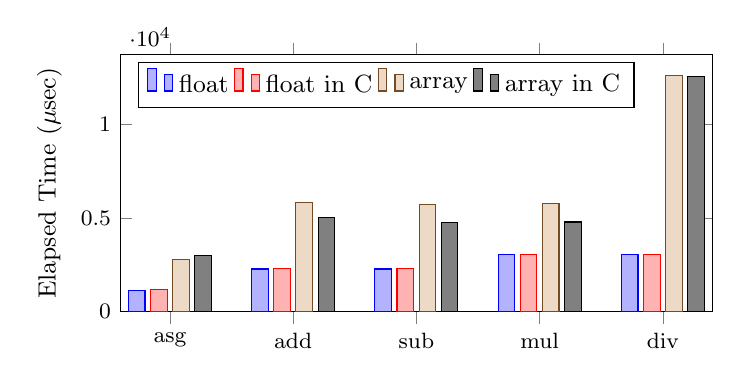
\begin{tikzpicture}
\begin{axis}[
  ybar, bar width=6pt,
  ylabel=Elapsed Time ($\mu$sec),
  symbolic x coords={asg, add, sub, mul, div},
  legend pos=north west, legend columns=4]
\addplot coordinates
  {(asg, 1134.2) (add, 2277.2) (sub, 2271.8) (mul, 3034) (div, 3029.2)};
\addplot coordinates
  {(asg, 1168.6) (add, 2280.8) (sub, 2302.8) (mul, 3044) (div, 3039.2)};
\addplot coordinates
  {(asg, 2800.4) (add, 5823.2) (sub, 5733) (mul, 5792.2) (div, 12575)};
\addplot coordinates
  {(asg, 3000.4) (add, 5008.8) (sub, 4763.2) (mul, 4783.8) (div, 12519.6)};
\legend{float, float in C, array, array in C}
\end{axis}
\end{tikzpicture}

\caption{Comparison of float point arithmetics}
\label{fig:arith}
\end{figure}

\subsubsection{Tuple vs. Record}\label{sec:tuple_record}
{\em Tuple} and {\em Record} are two light-weight data types for encapsulating a
group of data. When translated to intermediate C code, tuple is transformed to
multiple dimensional array and record is transformed to the {\ic struct} type.
Following code illustrates the correspondence in translation of {\ic tuple}
type, {\ic record} type, and their nested constructions.

\begin{lstlisting}
    /* Chapel source */            /* C mapping */
    var tup: (int, int);           int tup[2];
    var nstTup: (tup, tup);        int nstTup[2][2];

    record Rec {var x, y: int;}    struct rec {int x, y;}
    record nstRec {                struct nstRec {
        var x, y: Rec; }               struct rec x, y; }
\end{lstlisting}

As described in \autoref{sec:md_datastruct}, both {\ic tuple} and {\ic
record} can be used to implement vector. \autoref{fig:1d_vector} and
\autoref{fig:2d_vector} show the manipulation performance of 1D and 2D vectors,
respectively. 2D vector is implemented by nested types. The number of vectors is
$10^6$ and we also compare them with a {\em direct C implementation} using array
and {\ic struct}. Results show that using {\ic tuple} has a potential indexing
overhead (up to 50\%) than using {\ic record}, and the increment of overhead by
using nested types is much higher comparing to direct C implementation.

\begin{figure}[t]
\centering
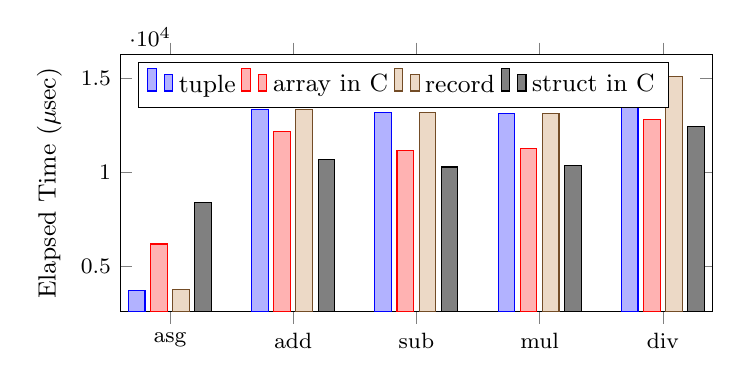
\begin{tikzpicture}
\begin{axis}[
  ybar, bar width=6pt,
  ylabel=Elapsed Time ($\mu$sec),
  symbolic x coords={asg, add, sub, mul, div},
  legend pos=north west, legend columns=4]
\addplot coordinates
  {(asg, 3733.8) (add, 13373.6) (sub, 13202.2) (mul, 13135) (div, 15143.4)};
\addplot coordinates
  {(asg, 6198.2) (add, 12207.6) (sub, 11178) (mul, 11278.8) (div, 12806)};
\addplot coordinates
  {(asg, 3788.4) (add, 13375.2) (sub, 13210.4) (mul, 13145.2) (div, 15115.2)};
\addplot coordinates
  {(asg, 8392.8) (add, 10704.6) (sub, 10299.4) (mul, 10362.4) (div, 12472.4)};
\legend{tuple, array in C, record, struct in C}
\end{axis}
\end{tikzpicture}

\caption{Performance of manipulations on 1D-vectors}
\label{fig:1d_vector}
\end{figure}

\begin{figure}[t]
\centering
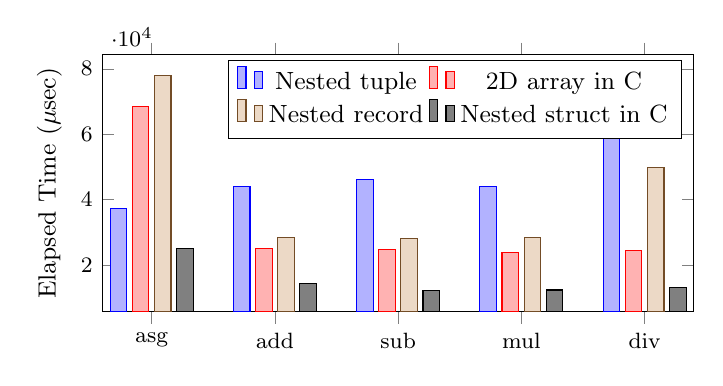
\begin{tikzpicture}
\begin{axis}[
  ybar, bar width=6pt,
  ylabel=Elapsed Time ($\mu$sec),
  symbolic x coords={asg, add, sub, mul, div},
  legend columns=2]
\addplot coordinates
  {(asg, 37227.6) (add, 43990.8) (sub, 46055.6) (mul, 43937.6) (div, 59695)};
\addplot coordinates
  {(asg, 68454.2) (add, 25028.8) (sub, 24933.2) (mul, 23775.2) (div, 24469.8)};
\addplot coordinates
  {(asg, 77836) (add, 28498) (sub, 28265.8) (mul, 28566.2) (div, 49820.6)};
\addplot coordinates
  {(asg, 25209.2) (add, 14292) (sub, 12311.4) (mul, 12413.6) (div, 13181)};
\legend{Nested tuple, 2D array in C, Nested record, Nested struct in C}
\end{axis}
\end{tikzpicture}

\caption{Performance of manipulation on 2D-vectors}
\label{fig:2d_vector}
\end{figure}

\subsection{Domain Indexing}
In Chapel, domain is classified as {\em rectangular domain} and {\em
irregular/associative domain}~\cite{chapelspec}. Rectangular domain describes
multidimensional rectangular index sets, and irregular domain is like
dictionary-style array which can use arbitrary type as index.

To study the performance of domain reference, we compare the throughput of
manipulation on arrays that are defined by rectangular domain and associate
domain. The size of all arrays is set to $10^6$, and the length of a
$n$-dimensional array is $10^{6/n}$. \autoref{fig:array} presents the
experimental results. Generally, using regular domain is much more efficient
(hundreds times faster) than using associate domain because regular domain
typically requires $O(1)$ space~\cite{chapelspec}.
\begin{figure}[t]
\centering
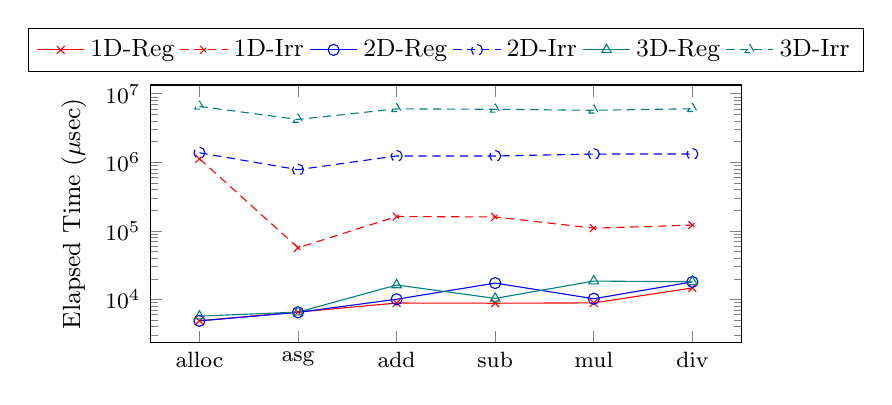
\begin{tikzpicture}
\begin{axis}[
  ymode=log,
  ylabel=Elapsed Time ($\mu$sec),
  symbolic x coords={alloc, asg, add, sub, mul, div},
  legend style={at={(0.5, 1.05)}, anchor=south, legend columns=6}]]
% 1D-Rec
\addplot[mark=x, color=red] coordinates
  {(alloc, 4878.8) (asg, 6555.2) (add, 8872.4) (sub, 8819.2) (mul, 8912.8) 
   (div,14743.4)};
% 1D-Irr
\addplot[mark=x, color=red, style=densely dashed] coordinates
  {(alloc, 1130004.8) (asg, 56809) (add, 162065.2) (sub, 159844) (mul, 109623)
   (div, 121578.4)};
% 2D-Rec
\addplot[mark=o, color=blue] coordinates
  {(alloc, 4873.8) (asg, 6490.8) (add, 10068) (sub, 17344.4) (mul, 10250.8)
   (div, 18036.8)};
% 2D-Irr
\addplot[mark=o, color=blue, style=densely dashed] coordinates
  {(alloc, 1377234.2) (asg, 781581.4) (add, 1238850.4) (sub, 1238424.4)
   (mul, 1319992) (div, 1324668)};
% 3D-Rec
\addplot[mark=triangle, color=teal] coordinates
  {(alloc, 5708.4) (asg, 6549.8) (add, 16246.4) (sub, 10368.6) (mul, 18559)
   (div, 18087.8)};
% 3D-Irr
\addplot[mark=triangle, color=teal, style=densely dashed] coordinates
  {(alloc, 6544416) (asg, 4218638) (add, 6025574) (sub, 5937296) (mul, 5747632)
   (div, 6049830)};
\legend{1D-Reg, 1D-Irr, 2D-Reg, 2D-Irr, 3D-Reg, 3D-Irr}
\end{axis}
\end{tikzpicture}

\caption{Indexing performance of arrays with different domains}
\label{fig:array}
\end{figure}

\subsection{Nested For Loop}\label{sec:nested_loop}
The nested loop is common in scientific calculation, and it can be constructed
using a {\em nested iteration} or {\em zipper iteration} in Chapel. But when the
inner loop depends on the outer loop, the iteration can only use the nested way
because the {\em range literal} is evaluated at once before iterations (see
example below).
\begin{lstlisting}
    // Nested iteration
    for i in [1..I] do  // Inner loop depends on outer loop
      for j in [1..I-1] { .. } 

    // Zipper iteration
    for (i, j) in [1..I, 1..J] do { ... }    // OK
    for (i, j) in [1..I, 1..I-1] do { ... }  // NG
\end{lstlisting}

\autoref{fig:loop} shows the elapsed time of conducing $10^6$ times of
accumulation by using different {\ic for}/{\ic while} constructions. Here,
``{\ic for-for}'' stands for a nested iteration and ``{\ic for2}'' stands for a
zipper iteration. For a $n$-level nested loops, each level is iterated for
$10^{6/n}$ times.
\begin{figure*}[t]
\centering
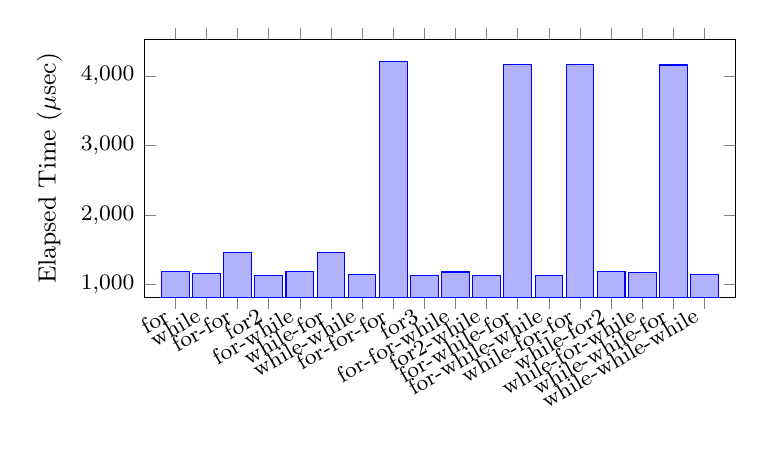
\begin{tikzpicture}
\begin{axis}[ybar,
  x tick label style={rotate=30, anchor=east},
  ylabel=Elapsed Time ($\mu$sec),
  xmin=0, xmax=19,
  xtick={1,2,3,4,5,6,7,8,9,10,11,12,13,14,15,16,17,18},
  xticklabels={for, while, for-for, for2, for-while, while-for,
  while-while, for-for-for, for3, for-for-while, for2-while,
  for-while-for, for-while-while, while-for-for, while-for2, while-for-while,
  while-while-for, while-while-while}]
\addplot coordinates
{(1, 1183) (2, 1166.2) (3, 1464)  (4, 1135.4) (5, 1183) 
 (6, 1467.8) (7, 1145.2) (8, 4209.6) 
 (9, 1136.4) (10, 1182) (11, 1136)
 (12, 4165.6) (13, 1129.4) (14, 4156)
 (15, 1184.8) (16, 1179.4) (17, 4155)
 (18, 1144.6)};
\end{axis}
\end{tikzpicture}

\caption{Performance comparison of traversing various nested loops}
\label{fig:loop}
\end{figure*}

It is clear that the overhead is non-trivial when {\ic for} exists in inner
loops. Following intermediate C code shows that a {\ic for} loop in Chapel is
translated into a {\ic while} loop surrounded by a pair of domain constructor
and destructor procedures which are also iterated by outer loops.

\begin{lstlisting}
    // Transformed C code of the for loop
    chpl__buildDomainExpr2(&loop_domain, ...);
    while (loop_domain) { ... }
    chpl__autoDestroy2(loop_variable, ...);
\end{lstlisting}

Thus, there are three ways to overcome this problem by preventing compiler from
inserting the domain construction procedures.
\begin{itemize}
  \item Define an {\em iterator} by using {\ic iter} function~\cite{chapelspec},
  which preserves the semantics of data parallelism in the {\ic forall}
  loop\footnote{However, the parallel iterator is not available now. It will be
  supported in the future~\cite{chapelspec}.}. 
  \item Use the {\ic while} statement for inner loop, if the inner loop does not
  need to be executed in parallel.
  \item Use zipper iteration, if inner loop is independent of outer loop.
\end{itemize}

\subsection{Molecular Dynamics Applications}

\subsubsection{Serial Execution Performance}
\autoref{fig:fmm_serial} shows the performance of the serial version of
\ac{FMM}. Similar as evaluation results in previous sections, a Chapel program
generally achieves about 50\% of the performance of an identical C program.
Though not shown here, other simpler \ac{MD} programs with fewer array reference
can achieve about 60-70\% performance of the C implementation.

\begin{figure}[t]
\centering
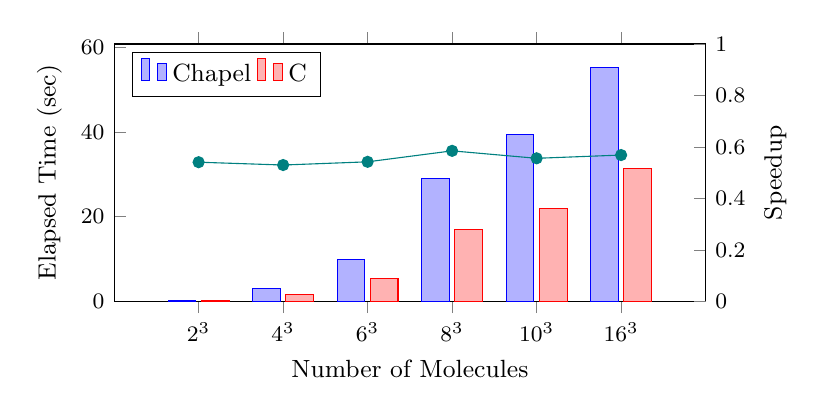
\begin{tikzpicture}
\begin{axis}[ybar, ylabel=Elapsed Time (sec), ymin=0, axis y line*=left,
  xlabel=Number of Molecules,
  xmin=0, xmax=7, xtick={1,2,3,4,5,6},
  xticklabels={$2^3$, $4^3$, $6^3$, $8^3$, $10^3$, $16^3$},
  legend pos=north west, legend columns=2]
\addplot coordinates
{(1, 0.1738) (2, 3.0888) (3, 9.93) (4, 28.9722) (5, 39.4486) (6, 55.2144)};
\addplot coordinates
{(1, 0.094) (2, 1.6366) (3, 5.385) (4, 16.9468) (5, 21.9326) (6, 31.3942)};
\legend{Chapel, C}
\end{axis}

\begin{axis}[xmin=0, xmax=7, ymin=0, ymax=1,
axis y line*=right, axis x line=none, ylabel=Speedup]
\addplot[mark=*, color=teal, update limits=false] coordinates
{(1, 0.54085) (2, 0.52984) (3, 0.54229) (4, 0.58493) (5, 0.55598) (6, 0.56859)};
\end{axis}
\end{tikzpicture}

\caption{Performance of serial \acs{FMM}}
\label{fig:fmm_serial}
\end{figure}

\subsubsection{Parallel Execution Performance}
To parallelize a serial program, parallel statements and synchronization are
inserted. Figure~\ref{fig:fmm_breakdown} shows the performance breakdown of
\ac{FMM} phases by a serial version and a parallelized version (but executed
serially) \ac{FMM} programs. For the most computation intensive part (\ie
{\ic multipoleCalc} phase), the parallelization can introduces 5 times of
overhead because lock is used in a heavy loop part.
\begin{figure}[t]
\centering
% huscs, N=32*32*32, numThreadsPerLocale=1, step=1
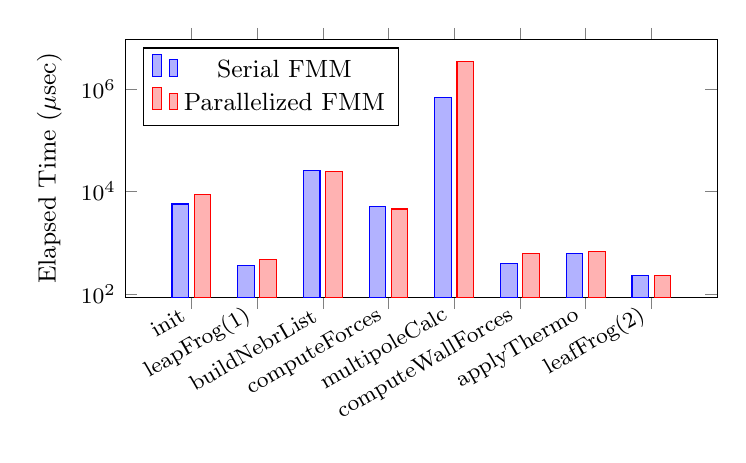
\begin{tikzpicture}
\begin{axis}[
  ymode=log, ybar, bar width=6pt,
  ylabel=Elapsed Time ($\mu$sec),
  xmin=0, xmax=9, xtick={1, 2, 3, 4, 5, 6, 7, 8},
  xticklabels={init, leapFrog(1), buildNebrList, computeForces, multipoleCalc,
    computeWallForces, applyThermo, leafFrog(2)},
  x tick label style={rotate=30, anchor=east},
  legend pos=north west, legend columns=1]
\addplot coordinates
  {(1, 5691) (2, 360) (3, 25388) (4, 5145) (5, 674491) (6, 385) (7, 603) 
   (8, 227)};
\addplot coordinates
  {(1, 8631) (2, 462) (3, 24151) (4, 4550) (5, 3480940) (6, 618) (7, 680) 
   (8, 231)};
\legend{Serial FMM, Parallelized FMM}
\end{axis}
\end{tikzpicture}

\caption{Serial performance breakdown of serial \ac{FMM} and parallelized \ac{FMM}}
\label{fig:fmm_breakdown}
\end{figure}

Figure~\ref{fig:fmm_scale} shows the scalability of parallel \ac{FMM} for
different number of threads and problem sizes.
Figure~\ref{fig:fmm_scale_breakdown} illustrates the scalability of each phase
for $N=32^3$.  For a small problem size (\eg $N=8^3$), the performance drops
down when the number of threads exceed 4 because there are less calculations for
long range interactions and the computation for short range is dominant. When
there are more molecules, which suggests larger space, the performance scales up
to 8 threads. However, the speedup only achieves 4 for 8 threads, this is
because an lock existing in {\ic multipoleCalc} phase leads to significant
overhead. We are currently developing a new algorithm for this phase to remove
the usage of lock.

\begin{figure}[t]
\centering
% huscs, steps=10
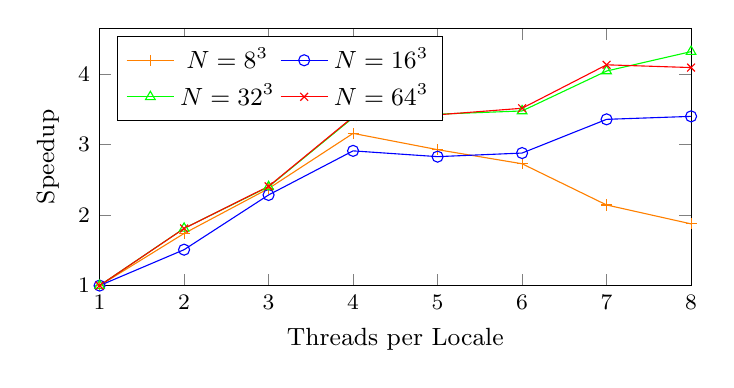
\begin{tikzpicture}
\begin{axis}[
  ylabel=Speedup, ymin=1,
  xmin=1, xmax=8, xtick={1, 2, 3, 4, 5, 6, 7, 8},
  xlabel=Threads per Locale,
  legend pos=north west, legend columns=2]
% N=8**3
\addplot[mark=+, color=orange] coordinates
  % 0.24  0.138 0.101 0.076 0.082 0.088 0.112 0.128
  {(1, 1) (2, 1.739) (3, 2.376) (4, 3.158) (5, 2.927) (6, 2.727) 
   (7, 2.143) (8, 1.875)};
% N=16**3
\addplot[mark=o, color=blue] coordinates
  % 0.809 0.536 0.354 0.278 0.286 0.281 0.241 0.2380
  {(1, 1) (2, 1.509) (3, 2.285) (4, 2.910) (5, 2.828) (6, 2.879) 
   (7, 3.357) (8, 3.399)};
% N=32**3
\addplot[mark=triangle, color=green] coordinates
  % 34.859, 19.244, 14.521, 10.310, 10.163, 10.028, 8.625, 8.075
  {(1, 1) (2, 1.811) (3, 2.401) (4, 3.381) (5, 3.430) (6, 3.476) 
   (7, 4.042) (8, 4.317)};
% N=64**3, STEP=2
\addplot[mark=x, color=red] coordinates
  % 440.885 243.609 183.189 129.985 128.869 125.48  106.816 107.761
  {(1, 1) (2, 1.810) (3, 2.407) (4, 3.392) (5, 3.421) (6, 3.514) 
   (7, 4.13) (8, 4.091)};
\legend{$N=8^3$, $N=16^3$, $N=32^3$, $N=64^3$}
\end{axis}
\end{tikzpicture}

\caption{Scalability of parallelized \ac{FMM}}
\label{fig:fmm_scale}
\end{figure}

\begin{figure}[t]
\centering
% huscs, N=32*32*32, numThreadsPerLocale=1,2,3,..,8, step=1
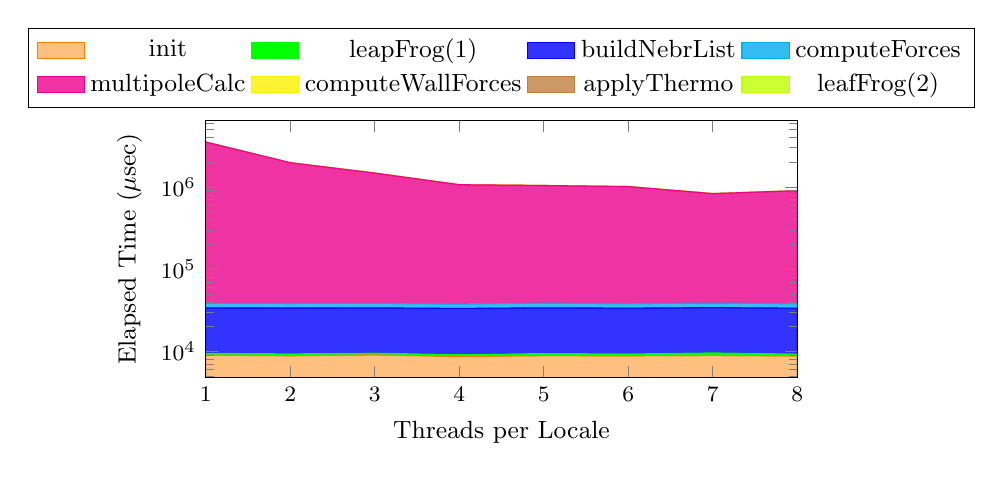
\begin{tikzpicture}
\begin{axis}[
  stack plots=y, area style, enlarge x limits=false,
  ymode=log,
  ylabel=Elapsed Time ($\mu$sec),
  xmin=1, xmax=8, xtick={1, 2, 3, 4, 5, 6, 7, 8},
  xlabel=Threads per Locale,
  legend style={at={(0.5, 1.05)}, anchor=south, legend columns=4}]
\addplot[orange, fill=orange, fill opacity=0.5] coordinates % init
  {(1, 8989) (2, 8825) (3, 9045) (4, 8658) (5, 8850) (6, 8821) (7, 8914) 
   (8, 8783)} \closedcycle;
\addplot[green, fill=green] coordinates % leapFrog(1)
  {(1, 454) (2, 468) (3, 426) (4, 425) (5, 530) (6, 440) (7, 637) (8, 457)}
  \closedcycle;
\addplot[blue, fill=blue, fill opacity=0.8] coordinates % buildNebrList
  {(1, 24268) (2, 24276) (3, 24282) (4, 24134) (5, 24417) (6, 24213) (7, 24434) 
   (8, 24207)} \closedcycle;
\addplot[cyan, fill=cyan, fill opacity=0.8] coordinates % computeForce
  {(1, 4612) (2, 4618) (3, 4564) (4, 4528) (5, 4653) (6, 4581) (7, 4567) 
   (8, 4549)} \closedcycle;
\addplot[magenta, fill=magenta, fill opacity=0.8] coordinates % multipoleCalc
  {(1, 3480480) (2, 1932990) (3, 1434660) (4, 1025450) (5, 1000760) 
   (6, 970789) (7, 789904) (8, 861565)} \closedcycle;
\addplot[yellow, fill=yellow, fill opacity=0.8] coordinates % computeWallForce
  {(1, 727) (2, 840) (3, 738) (4, 659) (5, 509) (6, 619) (7, 811) (8, 450)}
  \closedcycle;
\addplot[brown, fill=brown, fill opacity=0.8] coordinates % applyThermo
  {(1, 647) (2, 724) (3, 798) (4, 690) (5, 670) (6, 679) (7, 906) (8, 649)}
  \closedcycle;
\addplot[lime, fill=lime, fill opacity=0.8] coordinates % leapFrog(2)
  {(1, 233) (2, 380) (3, 399) (4, 340) (5, 335) (6, 364) (7, 447) (8, 334)}
  \closedcycle;
\legend{init, leapFrog(1), buildNebrList, computeForces, multipoleCalc,
    computeWallForces, applyThermo, leafFrog(2)},
\end{axis}
\end{tikzpicture}

\caption{Parallel performance breakdown of parallelized \ac{FMM}}
\label{fig:fmm_scale_breakdown}
\end{figure}

\subsection{Source Lines of Code}
Figure~\ref{fig:loc} shows the head-to-head comparison of \ac{LOC} between
serial programs of our Chapel and original C implementation. Using Chapel saves
20-40\% effort to develop a program. Note that the parallel version of programs
in Chapel only introduce a small fraction of additional code. For example, our
parallelized \ac{FMM} program has only 3\% more lines of code than the serial
version, which demonstrates that expressive of describing parallelism by Chapel.

\begin{figure}[t]
\centering
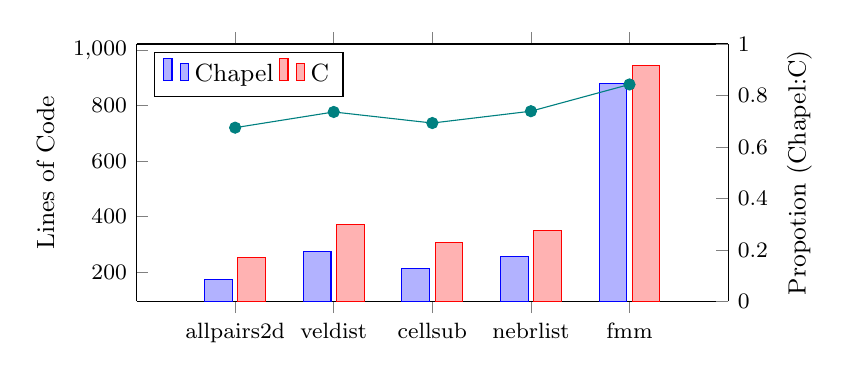
\begin{tikzpicture}
\begin{axis}[ybar, axis y line*=left,
  ylabel=Lines of Code, legend pos=north west, legend columns=2, xmin=0, xmax=6,
  xtick={1,2,3,4,5}, 
  xticklabels={allpairs2d, veldist, cellsub, nebrlist, fmm}]
\addplot plot coordinates
{(1, 171) (2, 273) (3, 212) (4, 257) (5, 880)};
\addplot plot coordinates
{(1, 253) (2, 371) (3, 306) (4, 348) (5, 945)};
\legend{Chapel, C}
\end{axis}

\begin{axis}[axis y line*=right,
  axis x line=none,
  ylabel=Propotion (Chapel:C),
  xmin=0, xmax=6, ymin=0, ymax=1]
\addplot[mark=*, color=teal] plot coordinates
{(1, 0.675) (2, 0.736) (3, 0.693) (4, 0.739) (5, 0.843)};
\end{axis}
\end{tikzpicture}

\caption{Comparison of lines of code of serial MD programs}
\label{fig:loc}
\end{figure}


\appendices
\section{Theoretical Fundamentals}
\subsection{Newtonian Dynamics}

\subsection{Hamiltonian Dynamics}

\section{Resources on Molecular Dynamics}
\subsection{MIT Lecture 3.320 Atomistic Computer Modeling of Materials}
This course uses the theory and application of atomistic computer simulations
to model, understand, and predict the properties of real materials. Specific
topics include: energy models from classical potentials to first-principles
approaches; density functional theory and the total-energy pseudo-potential
method; errors and accuracy of quantitative predictions: thermodynamic
ensembles, Monte Carlo sampling and molecular dynamics simulations; free energy
and phase transitions; fluctuations and transport properties; and
coarse-graining approaches and mesoscale models. The course employs case
studies from industrial applications of advanced materials to nanotechnology.
Several laboratories will give students direct experience with simulations of
classical force fields, electronic-structure approaches, molecular dynamics,
and Monte Carlo.

Both lecture
\href{http://ocw.mit.edu/courses/materials-science-and-engineering/3-320-atomistic-computer-modeling-of-materials-sma-5107-spring-2005/video-lectures}{videos}
and
\href{http://ocw.mit.edu/courses/materials-science-and-engineering/3-320-atomistic-computer-modeling-of-materials-sma-5107-spring-2005/lecture-notes}{notes}
are online available at the
\href{http://ocw.mit.edu/courses/materials-science-and-engineering/3-320-atomistic-computer-modeling-of-materials-sma-5107-spring-2005}{course
homepage}.  Particularly, the molecular dynamics has been discussed in lecture
13, 14, and 15.

\subsection{Molecular Dynamics on GPUs}
This \href{http://www.nvidia.com/object/molecular_dynamics.html}{portal site}
exhibits technical materials of using NVIDIA's \ac{GPU}
technique \ac{CUDA} for \ac{MD} simulation.

\subsection{Projects, Software, and Benchmarks}
\subsubsection{Projects}
\begin{itemize}
  \item \href{http://folding.stanford.edu}{Folding@home}: a distributed
  computing project to harness idle computers around the world to simulate
  milliseconds of folding time.
\end{itemize}

\subsubsection{Software}
\begin{itemize}
  \item \href{http://ambermd.org/gpus/}{AMBER 11}: NVIDIA \ac{GPU} Acceleration
  Support 
  
  \item \href{http://www.ks.uiuc.edu/Research/namd/}{NAMD}: a parallel
  molecular dynamics code designed for high-performance simulation of large
  biomolecular systems.
  
  \item \href{http://www.gromacs.org/}{Gromacs}: a versatile package to perform
  molecular dynamics.

  \item \href{http://www.ks.uiuc.edu/Research/vmd/}{VMD}: a molecular
  visualization program for displaying, animating, and analyzing large
  biomolecular systems using 3-D graphics and built-in scripting.

  \item \href{http://www.nwchem-sw.org/}{MWChem}: a comprehensive and scalable
  open-source solution for large scale molecular
  simulations~\cite{valiev10cpc}.
\end{itemize}

\subsubsection{Benchmarks}
\begin{itemize}
  \item \href{http://www.fisica.uniud.it/~ercolessi/mdbnch.html}{MDBNCH}: a
  molecular dynamics benchmark
\end{itemize}

% you can choose not to have a title for an appendix
% if you want by leaving the argument blank

% use section* for acknowledgement
\ifCLASSOPTIONcompsoc
  % The Computer Society usually uses the plural form
  \section*{Acknowledgments}
\else
  % regular IEEE prefers the singular form
  \section*{Acknowledgment}
\fi
This work is partially supported by JST, CREST through its research project:
``Highly Productive, High Performance Application Frameworks for Post 
Petascale Computing.''

\ifCLASSOPTIONcaptionsoff
  \newpage
\fi

% trigger a \newpage just before the given reference
% number - used to balance the columns on the last page
% adjust value as needed - may need to be readjusted if
% the document is modified later
%\IEEEtriggeratref{8}
% The "triggered" command can be changed if desired:
%\IEEEtriggercmd{\enlargethispage{-5in}}

% references section

\bibliographystyle{IEEEtran}
\bibliography{IEEEfull,mdoch}

% biography section
% 
% If you have an EPS/PDF photo (graphicx package needed) extra braces are
% needed around the contents of the optional argument to biography to prevent
% the LaTeX parser from getting confused when it sees the complicated
% \includegraphics command within an optional argument. (You could create
% your own custom macro containing the \includegraphics command to make things
% simpler here.)
%\begin{biography}[{\includegraphics[width=1in,height=1.25in,clip,keepaspectratio]{mshell}}]{Michael Shell}
% or if you just want to reserve a space for a photo:

%\begin{IEEEbiography}{Michael Shell}
%Biography text here.
%\end{IEEEbiography}

% insert where needed to balance the two columns on the last page with
% biographies
%\newpage

%\begin{IEEEbiographynophoto}{Jane Doe}
%Biography text here.
%\end{IEEEbiographynophoto}

% You can push biographies down or up by placing
% a \vfill before or after them. The appropriate
% use of \vfill depends on what kind of text is
% on the last page and whether or not the columns
% are being equalized.

%\vfill

% Can be used to pull up biographies so that the bottom of the last one
% is flush with the other column.
%\enlargethispage{-5in}

\end{document}


%%% TEMPLATE MEMO %%%

% An example of a floating figure using the graphicx package.
% Note that \label must occur AFTER (or within) \caption.
% For figures, \caption should occur after the \includegraphics.
% Note that IEEEtran v1.7 and later has special internal code that
% is designed to preserve the operation of \label within \caption
% even when the captionsoff option is in effect. However, because
% of issues like this, it may be the safest practice to put all your
% \label just after \caption rather than within \caption{}.
%
% Reminder: the "draftcls" or "draftclsnofoot", not "draft", class
% option should be used if it is desired that the figures are to be
% displayed while in draft mode.
%
%\begin{figure}[!t]
%\centering
%\includegraphics[width=2.5in]{myfigure}
% where an .eps filename suffix will be assumed under latex, 
% and a .pdf suffix will be assumed for pdflatex; or what has been declared
% via \DeclareGraphicsExtensions.
%\caption{Simulation Results}
%\label{fig_sim}
%\end{figure}

% Note that IEEE typically puts floats only at the top, even when this
% results in a large percentage of a column being occupied by floats.
% However, the Computer Society has been known to put floats at the bottom.


% An example of a double column floating figure using two subfigures.
% (The subfig.sty package must be loaded for this to work.)
% The subfigure \label commands are set within each subfloat command, the
% \label for the overall figure must come after \caption.
% \hfil must be used as a separator to get equal spacing.
% The subfigure.sty package works much the same way, except \subfigure is
% used instead of \subfloat.
%
%\begin{figure*}[!t]
%\centerline{\subfloat[Case I]\includegraphics[width=2.5in]{subfigcase1}%
%\label{fig_first_case}}
%\hfil
%\subfloat[Case II]{\includegraphics[width=2.5in]{subfigcase2}%
%\label{fig_second_case}}}
%\caption{Simulation results}
%\label{fig_sim}
%\end{figure*}
%
% Note that often IEEE papers with subfigures do not employ subfigure
% captions (using the optional argument to \subfloat), but instead will
% reference/describe all of them (a), (b), etc., within the main caption.


% An example of a floating table. Note that, for IEEE style tables, the 
% \caption command should come BEFORE the table. Table text will default to
% \footnotesize as IEEE normally uses this smaller font for tables.
% The \label must come after \caption as always.
%
%\begin{table}[!t]
%% increase table row spacing, adjust to taste
%\renewcommand{\arraystretch}{1.3}
% if using array.sty, it might be a good idea to tweak the value of
% \extrarowheight as needed to properly center the text within the cells
%\caption{An Example of a Table}
%\label{table_example}
%\centering
%% Some packages, such as MDW tools, offer better commands for making tables
%% than the plain LaTeX2e tabular which is used here.
%\begin{tabular}{|c||c|}
%\hline
%One & Two\\
%\hline
%Three & Four\\
%\hline
%\end{tabular}
%\end{table}


% Note that IEEE does not put floats in the very first column - or typically
% anywhere on the first page for that matter. Also, in-text middle ("here")
% positioning is not used. Most IEEE journals use top floats exclusively.
% However, Computer Society journals sometimes do use bottom floats - bear
% this in mind when choosing appropriate optional arguments for the
% figure/table environments.
% Note that, LaTeX2e, unlike IEEE journals, places footnotes above bottom
% floats. This can be corrected via the \fnbelowfloat command of the
% stfloats package.

